
\documentclass[a4paper,11pt]{article}
\usepackage[a4paper, margin=8em]{geometry}

% usa i pacchetti per la scrittura in italiano
\usepackage[french,italian]{babel}
\usepackage[T1]{fontenc}
\usepackage[utf8]{inputenc}
\frenchspacing 

% usa i pacchetti per la formattazione matematica
\usepackage{amsmath, amssymb, amsthm, amsfonts}

% usa altri pacchetti
\usepackage{gensymb}
\usepackage{hyperref}
\usepackage{standalone}

\usepackage{colortbl}

\usepackage{xstring}
\usepackage{karnaugh-map}

% imposta il titolo
\title{Electronics for Embedded Systems notes}
\author{Luca Seggiani}
\date{2026}

% spaziatura liste
\usepackage{enumitem}
\setlist[itemize]{noitemsep, topsep=4pt, partopsep=0pt, parsep=2pt, leftmargin=*}
\setlist[enumerate]{noitemsep, topsep=4pt, partopsep=0pt, parsep=2pt, leftmargin=*}

% imposta lo stile
% usa helvetica
\usepackage[scaled]{helvet}
% usa palatino
\usepackage{palatino}
% usa un font monospazio guardabile
\usepackage{lmodern}

\renewcommand{\rmdefault}{ppl}
\renewcommand{\sfdefault}{phv}
\renewcommand{\ttdefault}{lmtt}

% circuiti
\usepackage{circuitikz}
\usetikzlibrary{babel}

% testo cerchiato
\newcommand*\circled[1]{\tikz[baseline=(char.base)]{
            \node[shape=circle,draw,inner sep=2pt] (char) {#1};}}

% disponi il titolo
\makeatletter
\renewcommand{\maketitle} {
	\begin{center} 
		\begin{minipage}[t]{.8\textwidth}
			\textsf{\huge\bfseries \@title} 
		\end{minipage}%
		\begin{minipage}[t]{.2\textwidth}
			\raggedleft \vspace{-1.65em}
			\textsf{\small \@author} \vfill
			\textsf{\small \@date}
		\end{minipage}
		\par
	\end{center}

	\thispagestyle{empty}
	\pagestyle{fancy}
}
\makeatother

% disponi teoremi
\usepackage{tcolorbox}
\newtcolorbox[auto counter, number within=section]{theorem}[2][]{%
	colback=blue!10, 
	colframe=blue!40!black, 
	sharp corners=northwest,
	fonttitle=\sffamily\bfseries, 
	title=Theorem~\thetcbcounter: #2, 
	#1
}

% disponi definizioni
\newtcolorbox[auto counter, number within=section]{definition}[2][]{%
	colback=red!10,
	colframe=red!40!black,
	sharp corners=northwest,
	fonttitle=\sffamily\bfseries,
	title=Definition~\thetcbcounter: #2,
	#1
}

% disponi codice
\usepackage{listings}
\usepackage[table]{xcolor}

\definecolor{codegreen}{rgb}{0,0.6,0}
\definecolor{codegray}{rgb}{0.5,0.5,0.5}
\definecolor{codepurple}{rgb}{0.58,0,0.82}
\definecolor{backcolour}{rgb}{0.95,0.95,0.92}

\lstdefinestyle{codestyle}{
		backgroundcolor=\color{black!5}, 
		commentstyle=\color{codegreen},
		keywordstyle=\bfseries\color{magenta},
		numberstyle=\sffamily\tiny\color{black!60},
		stringstyle=\color{green!50!black},
		basicstyle=\ttfamily\footnotesize,
		breakatwhitespace=false,         
		breaklines=true,                 
		captionpos=b,                    
		keepspaces=true,                 
		numbers=left,                    
		numbersep=5pt,                  
		showspaces=false,                
		showstringspaces=false,
		showtabs=false,                  
		tabsize=2
}

\lstdefinestyle{shellstyle}{
		backgroundcolor=\color{black!5}, 
		basicstyle=\ttfamily\footnotesize\color{black}, 
		commentstyle=\color{black}, 
		keywordstyle=\color{black},
		numberstyle=\color{black!5},
		stringstyle=\color{black}, 
		showspaces=false,
		showstringspaces=false, 
		showtabs=false, 
		tabsize=2, 
		numbers=none, 
		breaklines=true
}

\lstdefinelanguage{x86}{ 
  keywords={AAA, AAD, AAM, AAS, ADC, ADCB, ADCW, ADCL, ADD, ADDB, ADDW, ADDL, AND, ANDB, ANDW, ANDL,
        ARPL, BOUND, BSF, BSFL, BSFW, BSR, BSRL, BSRW, BSWAP, BT, BTC, BTCB, BTCW, BTCL, BTR, 
        BTRB, BTRW, BTRL, BTS, BTSB, BTSW, BTSL, CALL, CBW, CDQ, CLC, CLD, CLI, CLTS, CMC, CMP,
        CMPB, CMPW, CMPL, CMPS, CMPSB, CMPSD, CMPSW, CMPXCHG, CMPXCHGB, CMPXCHGW, CMPXCHGL,
        CMPXCHG8B, CPUID, CWDE, DAA, DAS, DEC, DECB, DECW, DECL, DIV, DIVB, DIVW, DIVL, ENTER,
        HLT, IDIV, IDIVB, IDIVW, IDIVL, IMUL, IMULB, IMULW, IMULL, IN, INB, INW, INL, INC, INCB,
        INCW, INCL, INS, INSB, INSD, INSW, INT, INT3, INTO, INVD, INVLPG, IRET, IRETD, JA, JAE,
        JB, JBE, JC, JCXZ, JE, JECXZ, JG, JGE, JL, JLE, JMP, JNA, JNAE, JNB, JNBE, JNC, JNE, JNG,
        JNGE, JNL, JNLE, JNO, JNP, JNS, JNZ, JO, JP, JPE, JPO, JS, JZ, LAHF, LAR, LCALL, LDS,
        LEA, LEAVE, LES, LFS, LGDT, LGS, LIDT, LMSW, LOCK, LODSB, LODSD, LODSW, LOOP, LOOPE,
        LOOPNE, LSL, LSS, LTR, MOV, MOVB, MOVW, MOVL, MOVSB, MOVSD, MOVSW, MOVSX, MOVSXB,
        MOVSXW, MOVSXL, MOVZX, MOVZXB, MOVZXW, MOVZXL, MUL, MULB, MULW, MULL, NEG, NEGB, NEGW,
        NEGL, NOP, NOT, NOTB, NOTW, NOTL, OR, ORB, ORW, ORL, OUT, OUTB, OUTW, OUTL, OUTSB, OUTSD,
        OUTSW, POP, POPL, POPW, POPB, POPA, POPAD, POPF, POPFD, PUSH, PUSHL, PUSHW, PUSHB, PUSHA, 
        RCLL, RCR, RCRB, RCRW, RCRL, RDMSR, RDPMC, RDTSC, REP, REPE, REPNE, RET, ROL, ROLB, ROLW,
        ROLL, ROR, RORB, RORW, RORL, SAHF, SAL, SALB, SALW, SALL, SAR, SARB, SARW, SARL, SBB,
        SBBB, SBBW, SBBL, SCASB, SCASD, SCASW, SETA, SETAE, SETB, SETBE, SETC, SETE, SETG, SETGE,
        SETL, SETLE, SETNA, SETNAE, SETNB, SETNBE, SETNC, SETNE, SETNG, SETNGE, SETNL, SETNLE,
        SETNO, SETNP, SETNS, SETNZ, SETO, SETP, SETPE, SETPO, SETS, SETZ, SGDT, SHL, SHLB, SHLW,
        SHLL, SHLD, SHR, SHRB, SHRW, SHRL, SHRD, SIDT, SLDT, SMSW, STC, STD, STI, STOSB, STOSD,
        STOSW, STR, SUB, SUBB, SUBW, SUBL, TEST, TESTB, TESTW, TESTL, VERR, VERW, WAIT, WBINVD,
        XADD, XADDB, XADDW, XADDL, XCHG, XCHGB, XCHGW, XCHGL, XLAT, XLATB, XOR, XORB, XORW, XORL},
  keywordstyle=\color{blue}\bfseries,
  ndkeywordstyle=\color{darkgray}\bfseries,
  identifierstyle=\color{black},
  sensitive=false,
  comment=[l]{\#},
  morecomment=[s]{/*}{*/},
  commentstyle=\color{purple}\ttfamily,
  stringstyle=\color{red}\ttfamily,
  morestring=[b]',
  morestring=[b]"
}

\lstdefinelanguage{riscv}{
  keywords={
    LUI, AUIPC,
    JAL, JALR,
    BEQ, BNE, BLT, BGE, BLTU, BGEU,
    LB, LH, LW, LBU, LHU, LD,
    SB, SH, SW, SD,
    ADDI, SLTI, SLTIU, XORI, ORI, ANDI,
    SLLI, SRLI, SRAI,
    ADD, SUB, SLL, SLT, SLTU, XOR, SRL, SRA, OR, AND,
    ADDIW, SLLIW, SRLIW, SRAIW,
    ADDW, SUBW, SLLW, SRLW, SRAW,
    MUL, MULH, MULHSU, MULHU, DIV, DIVU, REM, REMU,
    MULW, DIVW, DIVUW, REMW, REMUW,
    LR.W, SC.W, AMOSWAP.W, AMOADD.W, AMOXOR.W,
    AMOAND.W, AMOOR.W, AMOMIN.W, AMOMAX.W,
    AMOMINU.W, AMOMAXU.W,
    LR.D, SC.D, AMOSWAP.D, AMOADD.D, AMOXOR.D,
    AMOAND.D, AMOOR.D, AMOMIN.D, AMOMAX.D,
    AMOMINU.D, AMOMAXU.D,
    FLW, FSW,
    FMADD.S, FMSUB.S, FNMSUB.S, FNMADD.S,
    FADD.S, FSUB.S, FMUL.S, FDIV.S, FSQRT.S,
    FSGNJ.S, FSGNJN.S, FSGNJX.S,
    FMIN.S, FMAX.S,
    FCVT.W.S, FCVT.WU.S, FCVT.S.W, FCVT.S.WU,
    FMV.X.W, FMV.W.X,
    FEQ.S, FLT.S, FLE.S,
    FLD, FSD,
    FMADD.D, FMSUB.D, FNMSUB.D, FNMADD.D,
    FADD.D, FSUB.D, FMUL.D, FDIV.D, FSQRT.D,
    FSGNJ.D, FSGNJN.D, FSGNJX.D,
    FMIN.D, FMAX.D,
    FCVT.W.D, FCVT.WU.D, FCVT.D.W, FCVT.D.WU,
    FCVT.S.D, FCVT.D.S,
    FMV.X.D, FMV.D.X,
    FEQ.D, FLT.D, FLE.D,
    CSRRW, CSRRS, CSRRC,
    CSRRWI, CSRRSI, CSRRCI,
    FENCE.I,
    FENCE,
    ECALL, EBREAK,
    MRET, SRET, URET,
    WFI,
    SFENCE.VMA,
    NOP, LI, LA, MV,
    NOT, NEG, NEGW,
    SEQZ, SNEZ, SLTZ, SGTZ,
    BEQZ, BNEZ, BLEZ, BGEZ, BLTZ, BGTZ,
    BGT, BLE, BGTU, BLEU,
    J, JR, RET,
    CALL, TAIL,
    RDINSTRET, RDCYCLE, RDTIME,
    CSRR, CSRW, CSRS, CSRC,
    CSRWI, CSRSI, CSRCI
  },
  keywordstyle=\color{blue}\bfseries,
  ndkeywordstyle=\color{darkgray}\bfseries,
  identifierstyle=\color{black},
  sensitive=false,
  comment=[l]{\#},
  morecomment=[s]{/*}{*/},
  commentstyle=\color{purple}\ttfamily,
  stringstyle=\color{red}\ttfamily,
  morestring=[b]',
  morestring=[b]"
}

\lstdefinelanguage{arm}{
  keywords={
    ADC, ADD, AND, BIC, CMN, CMP, EOR, MOV, MVN,
    RSB, RSC, SBC, SUB, TST, TEQ,
    MLA, MLS, MUL, SMLAL, SMULL, UMLAL, UMULL,
    QADD, QSUB, QDADD, QDSUB,
    QADD16, QADD8, QASX, QSAX,
    QSUB16, QSUB8, QSAX, QSUBADDX,
    ASR, LSL, LSR, ROR, RRX,
    B, BL, BX, BLX,
    BXJ,
    BEQ, BNE, BCS, BHS, BCC, BLO,
    BMI, BPL, BVS, BVC,
    BHI, BLS, BGE, BLT, BGT, BLE,
    BAL,
    LDR, LDRB, LDRH, LDRSB, LDRSH,
    LDRD, LDM, LDMIA, LDMIB, LDMDA, LDMDB,
    LDRT, LDRBT, LDRHT, LDRSBT, LDRSHT,
    STR, STRB, STRH, STRD,
    STM, STMIA, STMIB, STMDA, STMDB,
    STRT, STRBT, STRHT,
    PUSH, POP,
    SWP, SWPB,
    REV, REV16, REVSH,
    BFC, BFI, BFXIL, SBFX, UBFX,
    CLZ,
    LDREX, LDREXB, LDREXH, LDREXD,
    STREX, STREXB, STREXH, STREXD,
    DMB, DSB, ISB,
    MCR, MCRR, MRC, MRRC,
    MRS, MSR,
    CPS, SETEND, SVC, BKPT,
    CLREX, WFE, WFI, SEV,
    YIELD, NOP,
    VLDR, VSTR,
    VMOV, VABS, VNEG,
    VADD, VSUB, VMUL, VDIV,
    VMLA, VMLS, VNMLA, VNMLS, VNMUL,
    VMAX, VMIN,
    VSQRT,
    VCMP, VCMPE,
    VCVT,
    VCLZ, VCLS,
    VAND, VORR, VEOR, VBIC, VMVN,
    VLD1, VLD2, VLD3, VLD4,
    VST1, VST2, VST3, VST4,
    ADR, ADCS, ADDS, SUBS, MOVS, ANDS, ORRS, EORS
  },
  keywordstyle=\color{blue}\bfseries,
  ndkeywordstyle=\color{darkgray}\bfseries,
  identifierstyle=\color{black},
  sensitive=false,
  comment=[l]{@},
  morecomment=[l]{;},
  morecomment=[s]{/*}{*/},
  commentstyle=\color{purple}\ttfamily,
  stringstyle=\color{red}\ttfamily,
  morestring=[b]',
  morestring=[b]"
}

\lstset{style=codestyle, language=C}

% disponi sezioni
\usepackage{titlesec}

\titleformat{\section}
	{\sffamily\Large\bfseries} 
	{\thesection}{1em}{} 
\titleformat{\subsection}
	{\sffamily\large\bfseries}   
	{\thesubsection}{1em}{} 
\titleformat{\subsubsection}
	{\sffamily\normalsize\bfseries} 
	{\thesubsubsection}{1em}{}

% tikz
\usepackage{tikz}

% float
\usepackage{float}

% grafici
\usepackage{pgfplots}
\pgfplotsset{width=10cm,compat=1.9}

% disponi alberi
\usepackage{forest}

\forestset{
	rectstyle/.style={
		for tree={rectangle,draw,font=\large\sffamily}
	},
	roundstyle/.style={
		for tree={circle,draw,font=\large}
	}
}

% disponi algoritmi
\usepackage{algorithm}
\usepackage{algorithmic}
\makeatletter
\renewcommand{\ALG@name}{Algorithm}
\makeatother

% disponi numeri di pagina
\usepackage{fancyhdr}
\fancyhf{} 
\fancyfoot[L]{\sffamily{\thepage}}

\makeatletter
\fancyhead[L]{\raisebox{1ex}[0pt][0pt]{\sffamily{\@title \ \@date}}} 
\fancyhead[R]{\raisebox{1ex}[0pt][0pt]{\sffamily{\@author}}}
\makeatother

\begin{document}
% sezione (data)
\section{Lesson 30-09-26}

% stili pagina
\thispagestyle{empty}
\pagestyle{fancy}

% testo
Last lesson we finished up on sequential circuits, introducing the \textit{bistable circuit} and making it controllable via a pair of NOR ports (implementing an \textit{SR latch}).
Let's start again from there.

\textbf{\textsf{SR latch w/ enable}}: let's add enable circuitry to the SR latch.
Note that \textit{enable} here doesn't mean setting the output to high impedance (as in tristates), but making the network unresponsive to changes in the inputs.

The circuits we could get are the following:
\begin{center}
	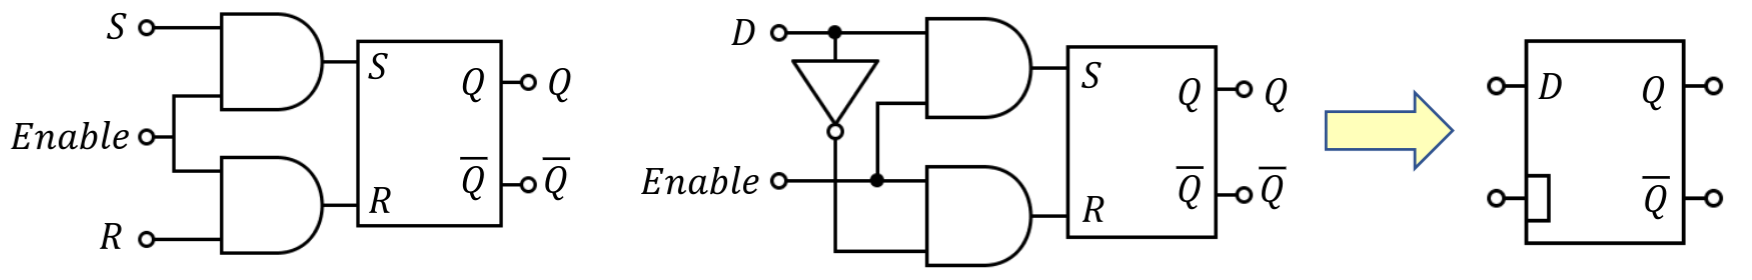
\includegraphics[scale=0.25]{../figures/sr_to_d_latch.png}
\end{center}

\textbf{\textsf{D latch}}: let's add enable circuitry to the SR latch.

Note that we decided to simplify the SR latch circuitry in the middle circuit, by setting $S$ to a data value $D$, and $R$ to its negation.
This allows us to build what's essentialy a \textbf{D latch} (last circuit in the row).

\textbf{\textsf{D flip flop}}: this is one last memory circuit we can build, which is even more convenient than the past two. 

\begin{center}
	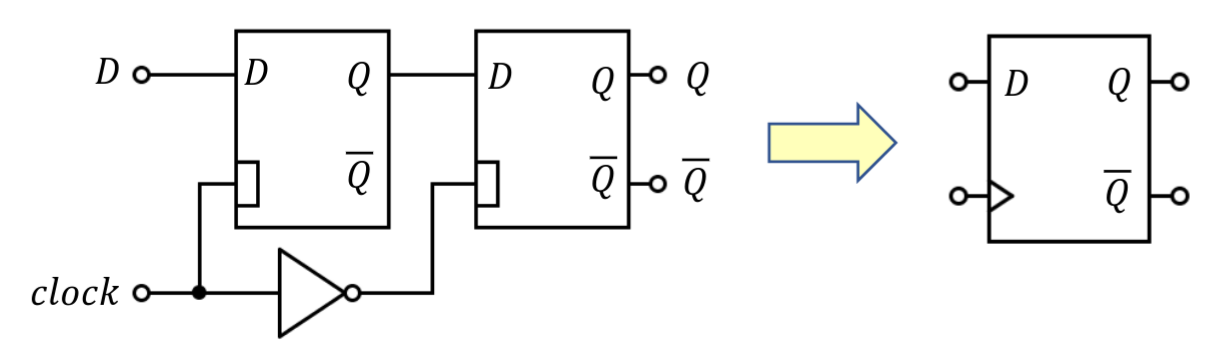
\includegraphics[scale=0.3]{../figures/d_flip_flop.png}
\end{center}

In the figure we note the master/slave implementation, but there are many others that can be built.
The idea of the D flip flop, no matter the implementation, is that the output value $Q$ follows the input $D$ \textit{only} on the rising edges of the clock signal.
This makes D flip flops non \textit{transparent}: a change in the input isn't trasmitted directly to the output (but only transiently during clock rising edges): in other words, if the circuit oscillates, it oscillates synchronized to the clock.
This makes this circuit extremely useful in sequential networks as a memory element (for instance in \textit{registers}). 

\par\smallskip

\textbf{\textsf{Other characteristics}}: let's note other characteristics of sequential networks.

Firstly, when talking about flip-flops and latches, we note that there are usually other inputs provided:
\begin{itemize}
	\item \textbf{Asynchronous clear} (or \textbf{reset}): sets the output to 0, without waiting the active clock edge;
	\item \textbf{Asynchronous set}: sets the output to 1, without waiting the active clock edge;
	\item \textbf{Clock enable}: masks the clock input.
\end{itemize}
These signals are often active low.

Other important characteristics are the \textbf{timing specifications} of flip-flops:
\begin{center}
	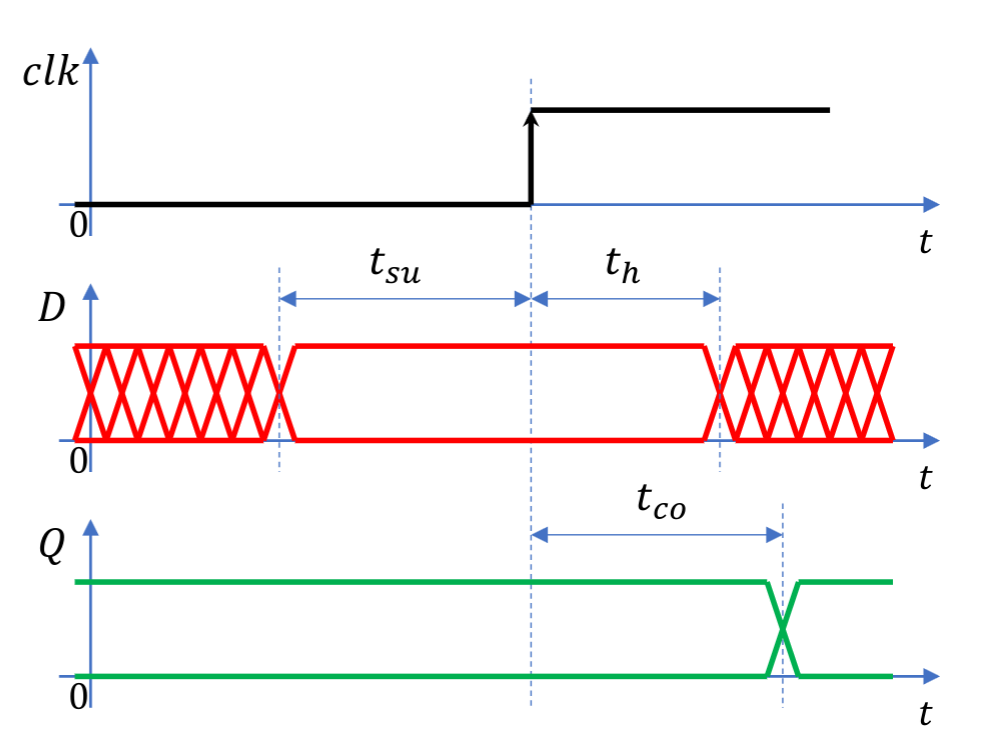
\includegraphics[scale=0.25]{../figures/flip_timings}
\end{center}
\begin{itemize}
	\item \textbf{Setup} time: the time the data input has to be stable \textit{before} the rising edge, for the flip-flop to correctly recognize its value;
	\item \textbf{Hold} time: the time the data input has to be stable \textit{after} the rising edge, for the flip-flop to correctly recognize its value;
	\item \textbf{Clock to output} time: the time the flip-flop takes to propagate its input to its output after a clock rising edge.
\end{itemize}
These values are often in the order of microseconds, and directly determine the maximum clock speeds we can achieve.

\textbf{\textsf{Registers}}: we introduced them, now let's look at them. A \textbf{register} in the electronics sense is nothing more than a combination of multiple flip-flops with a common clock and different data inputs.
This allows registers to store whole \textit{words} of data, of arbitrary size.
Let's look at a 3 bit register as an example.

\begin{center}
	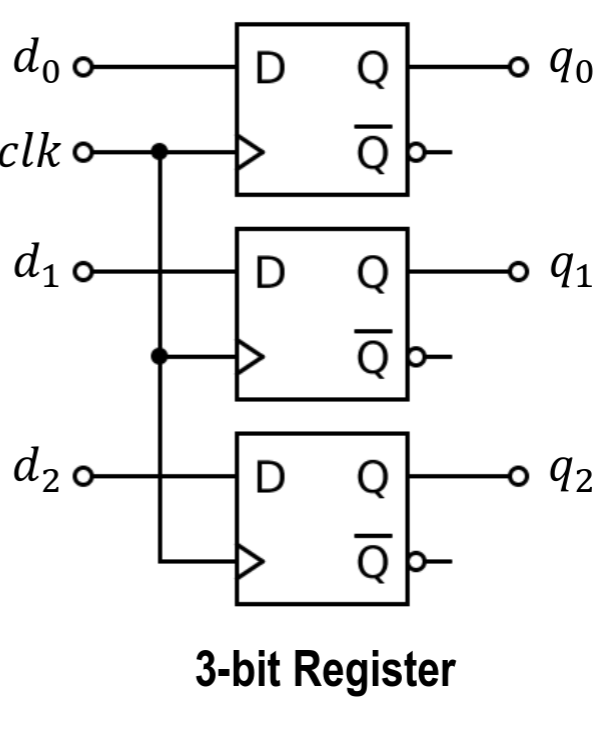
\includegraphics[scale=0.25]{../figures/register.png}
\end{center}

\textbf{\textsf{Shift register}}: a \textbf{shift} \textit{register}, often called a \textit{delay line}, is like a register which takes in a single bit of data and propagates it through a set of flip-flops.

\begin{center}
	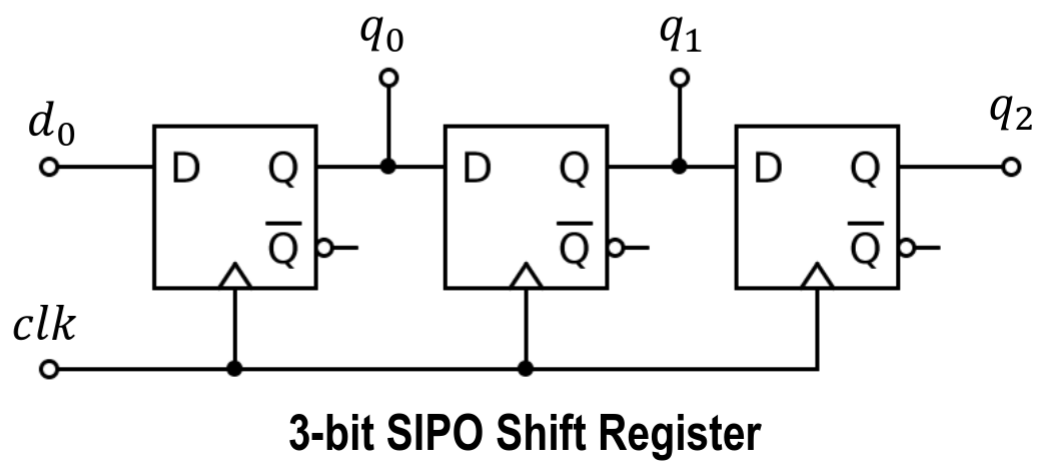
\includegraphics[scale=0.25]{../figures/shift_reg.png}
\end{center}

There are different kinds:
\begin{itemize}
	\item Serial In, Parallel Out (\textbf{SIPO});
	\item Parallel In, Serial Out (\textbf{PISO}): these need extra control inputs such as:
	\begin{itemize}
		\item Parallel Load (PL)
		\item Load Enable (LE)
	\end{itemize}
	\item Serial In, Serial Out (\textbf{SISO}): these often come with parallel out, as well.
\end{itemize}
All shift registers may have a shift enable signal.

\textbf{\textsf{Counter}}: there are 2 kinds of counters:
\begin{itemize}
	\item \textbf{Asynchronous counter}: the clock propagates from one FF to the next. This means that the most significant bits are updated later than least significant bits. This is undesirable as it entails \textit{data races} along the FFs. Still, it is the one we show an example of as it's the simplest;
	\item \textbf{Synchronous counter}: the same clock is provided to all FFs. Internal logic used to compute the input to each FF: this means all output bits are updated at the same time.
\end{itemize}

\begin{center}
	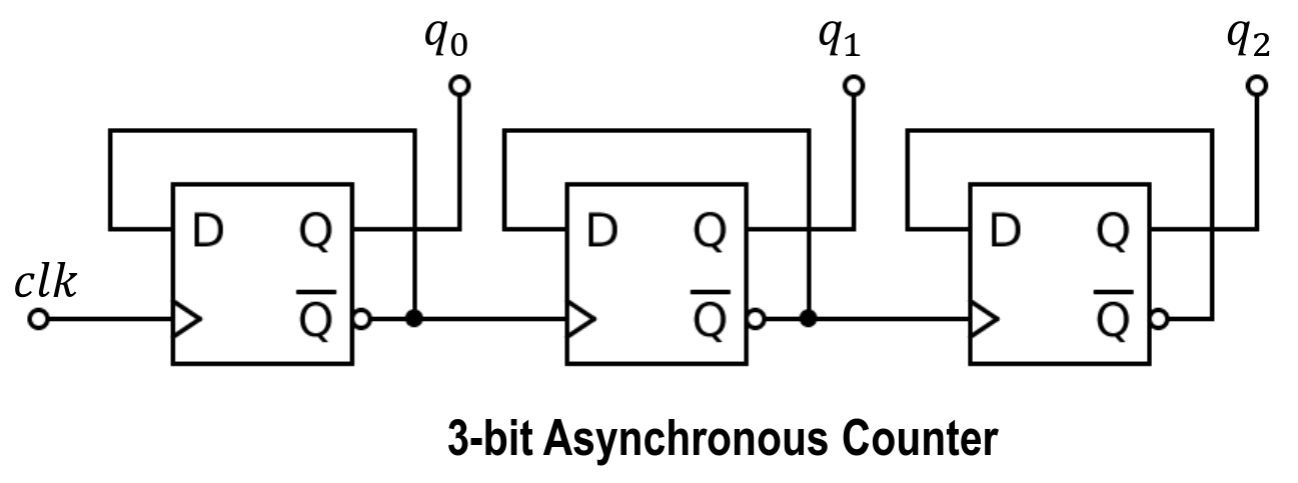
\includegraphics[scale=0.22]{../figures/async_count.png}
\end{center}

This being said, there are other characteristics which determine the behavior of a counter:
\begin{itemize}
	\item Up or Up/Down counters;
	\item Binary or Decade counters;
	\item Parallel Load to initialize counter value;
	\item Carry input and output to cascade counters;
	\item Asynchronous reset.
\end{itemize}

\par\smallskip

\textbf{\textsf{FSM}}: an \textbf{FSM} (\textit{Finite State Machine}) is a graph structure consisting of \textit{nodes}, corresponding to \textbf{states}, and \textit{edges}, corresponding to \textbf{state transistions}.
This way, a state machine defines all possible states of a digital systems and all the ways states can transition one to another.

A FSM description can also entail a network's outputs:
\begin{itemize}
	\item Edges may have output values (\textit{Mealy} model);
	\item States may have output values (\textit{Moore} model);
	\item Transitions are synchronized with an external clock signals (\textit{retarded} or \textit{synchronized} Mealy and Moore models).
\end{itemize}

State machines can formally be described via two truth tables:
\begin{itemize}
	\item One for \textit{state transitions} (next state), with respect to inputs and current state
	\item One for \textit{outputs}, with respect to current state (Moore) and inputs (Mealy).
\end{itemize}

\par\smallskip

\begin{center}
	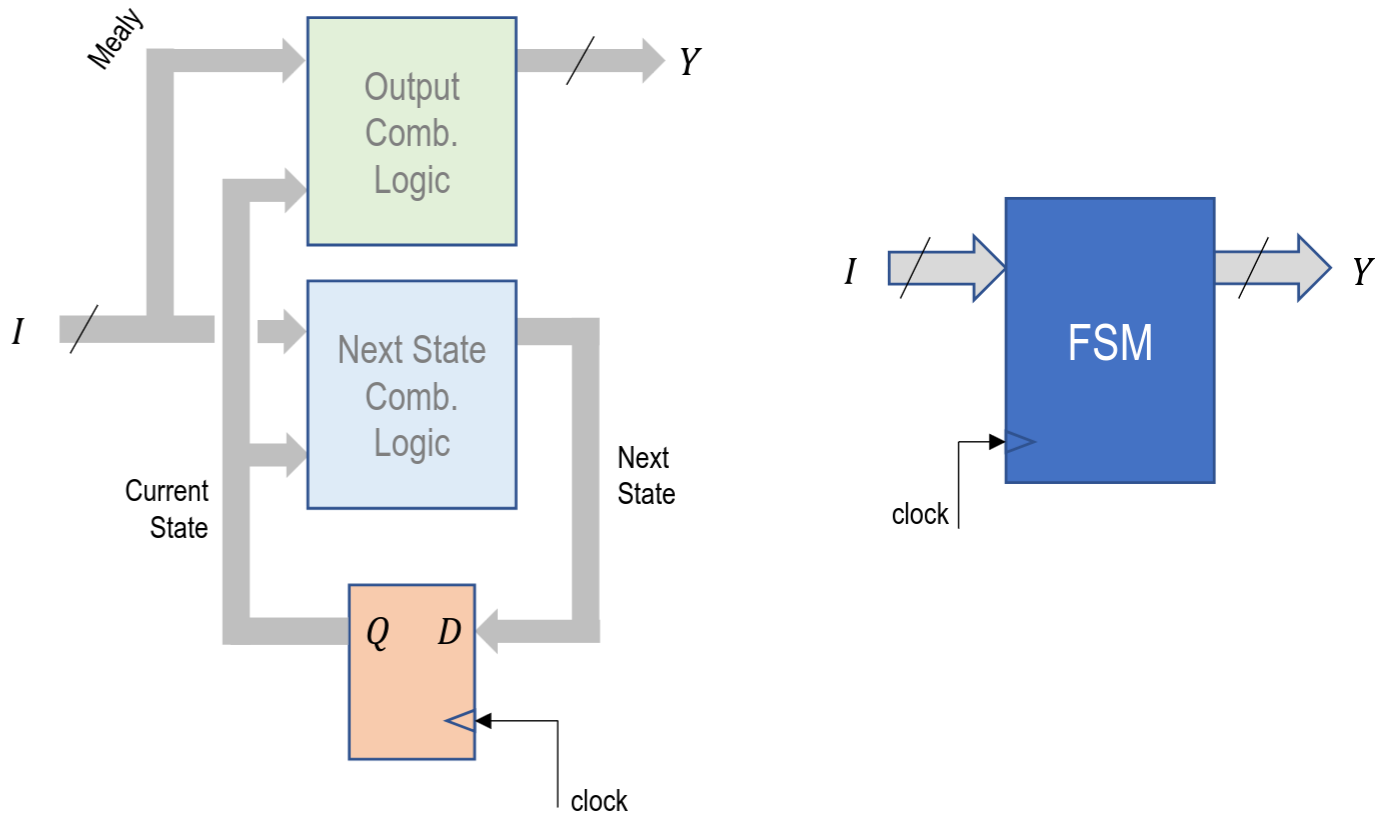
\includegraphics[scale=0.28]{../figures/fsm.png}
\end{center}

To implement a state machine as a circuit we first need the \textit{specification} of that state machine, which we said is either given by truth tables or state transition graphs.
Then, we can encode the internal state in a special register (the \textbf{STAR}, or \textit{STAtus Register}).
The STAR register has to be as big as the base-2 logarithm of the state space (in \textit{binary} encoding, as big as the state space for \textit{one-hot} encoding).

At this point the two truth tables become two combinational logic circuits:
\begin{itemize}
	\item One that takes in the current state (Moore) and/or the current inputs (Mealy) and returns the output of the network;
	\item One that takes the current state and the current inputs to determine the next state (which gets fed back to the STAR register).
\end{itemize}

\subsection{VHDL}

\textbf{VHDL} (\textit{VHSIC Hardware Description Language}) is a hardware description language that can model the behavior and structure of digital systems at multiple levels of abstraction, ranging from the system level down to that of logic gates.

\begin{itemize}
	\item It is used to \textit{describe} the structure and the behavior of a \textbf{digital system};
	\item The description can be used to \textit{simulate} and \textit{synthesize} a \textbf{digital circuit}.
\end{itemize}

The nice part of VHDL is that the syntax similar to a programming language.

The basic design element of a VHDL description is an \textbf{entity}, which is a design unit comprised of:
\begin{itemize}
	\item The \textbf{entity} specification, which acts as a black-box interface for the component:
		\begin{itemize}
			\item \textbf{Name} of entity;
			\item \textbf{Inputs};
			\item \textbf{Outputs};
			\item \textbf{In/out} ports;
		\end{itemize}
	\item The \textbf{architecture} specification, which describes the entity's behavior and/or internal structure. VHDL allows for a number of specification styles:
		\begin{itemize}
			\item \textbf{RTL} (\textit{Register Transfer Level}): uses \textit{concurrent signal assignments}.

				These are \textit{boolean expressions} assigned to a signal, executed in \textit{parallel}, so without any implied order. Not that lists of concurrent assignments are \textit{not} sequential in execution. High level operators such as arithmetic, logic and conditionals can be used;
			\item \textbf{Structural}: similar to a schematic diagram, but using a textual programming language.

				We first declare \textit{components}, then \textit{signals} to interconnect those components, and lastly \textit{map} signal and input/output ports to components. This allows for a hierarchical description of a circuit (Top/Down or Bottom/Up);
			\item \textbf{Behavioral}: uses a process, which is a sort of an endless loop, specified in a programming language-like way.

				In most cases it uses an implicit \textit{wait statement} on a \textit{sensitivity list}:
\begin{itemize}
	\item The process suspends when it reaches the end
	\item Resumes when any signal on the sensitivity list changes
\end{itemize}
Instructions in the process are, this time, in fact \textit{sequential}, but may still be implemented in parallel to increase performance if the compiler finds it is feasible.
Still, we note that signal assignments happen only \textit{at the end} of a certain process.
Higher level constructs such as if or case conditional expressions are available, variables can be defined and assignments to variables are immediate.
		\end{itemize}
\end{itemize}

\subsection{Introduction to embedded systems}

This course and the entire degree program are focused on \textbf{embedded systems}, so it might be natural to ask \textit{what} an embedded system even is.
An embedded system is an electronic system, that is a system made up of:
\begin{itemize}
	\item Hardware components;
	\item Software components;
	\item Communication systems.
\end{itemize}
designed to be part of a larger system, not necessarily electronic:
\begin{itemize}
	\item Vehicles (cars, planes, ...);
	\item Industrial systems;
	\item Home appliances.
\end{itemize}

This means that an embedded system:
\begin{itemize}
	\item Is, in fact, \textbf{embedded}, i.e. it lives in a larger environment;
	\item It should \textbf{react}, typically in real-time, to external stimuli;
	\item It is dedicated to a particular \textbf{application} (single task).
\end{itemize}

This gives designers the opportunity to highly optimize and adapt to different situations, in highly constrained environments. 

\textbf{Designing} embedded systems, in this regard, is difficult because:
\begin{itemize}
	\item The design space is extremely large;
	\item It requires skills from many very different domains;
	\item It requires to simultaneously optimize numerous design metrics.
\end{itemize}

\subsubsection{Architecture of an embedded system}

Let us look at the typical components of an embedded system:
\begin{center}
	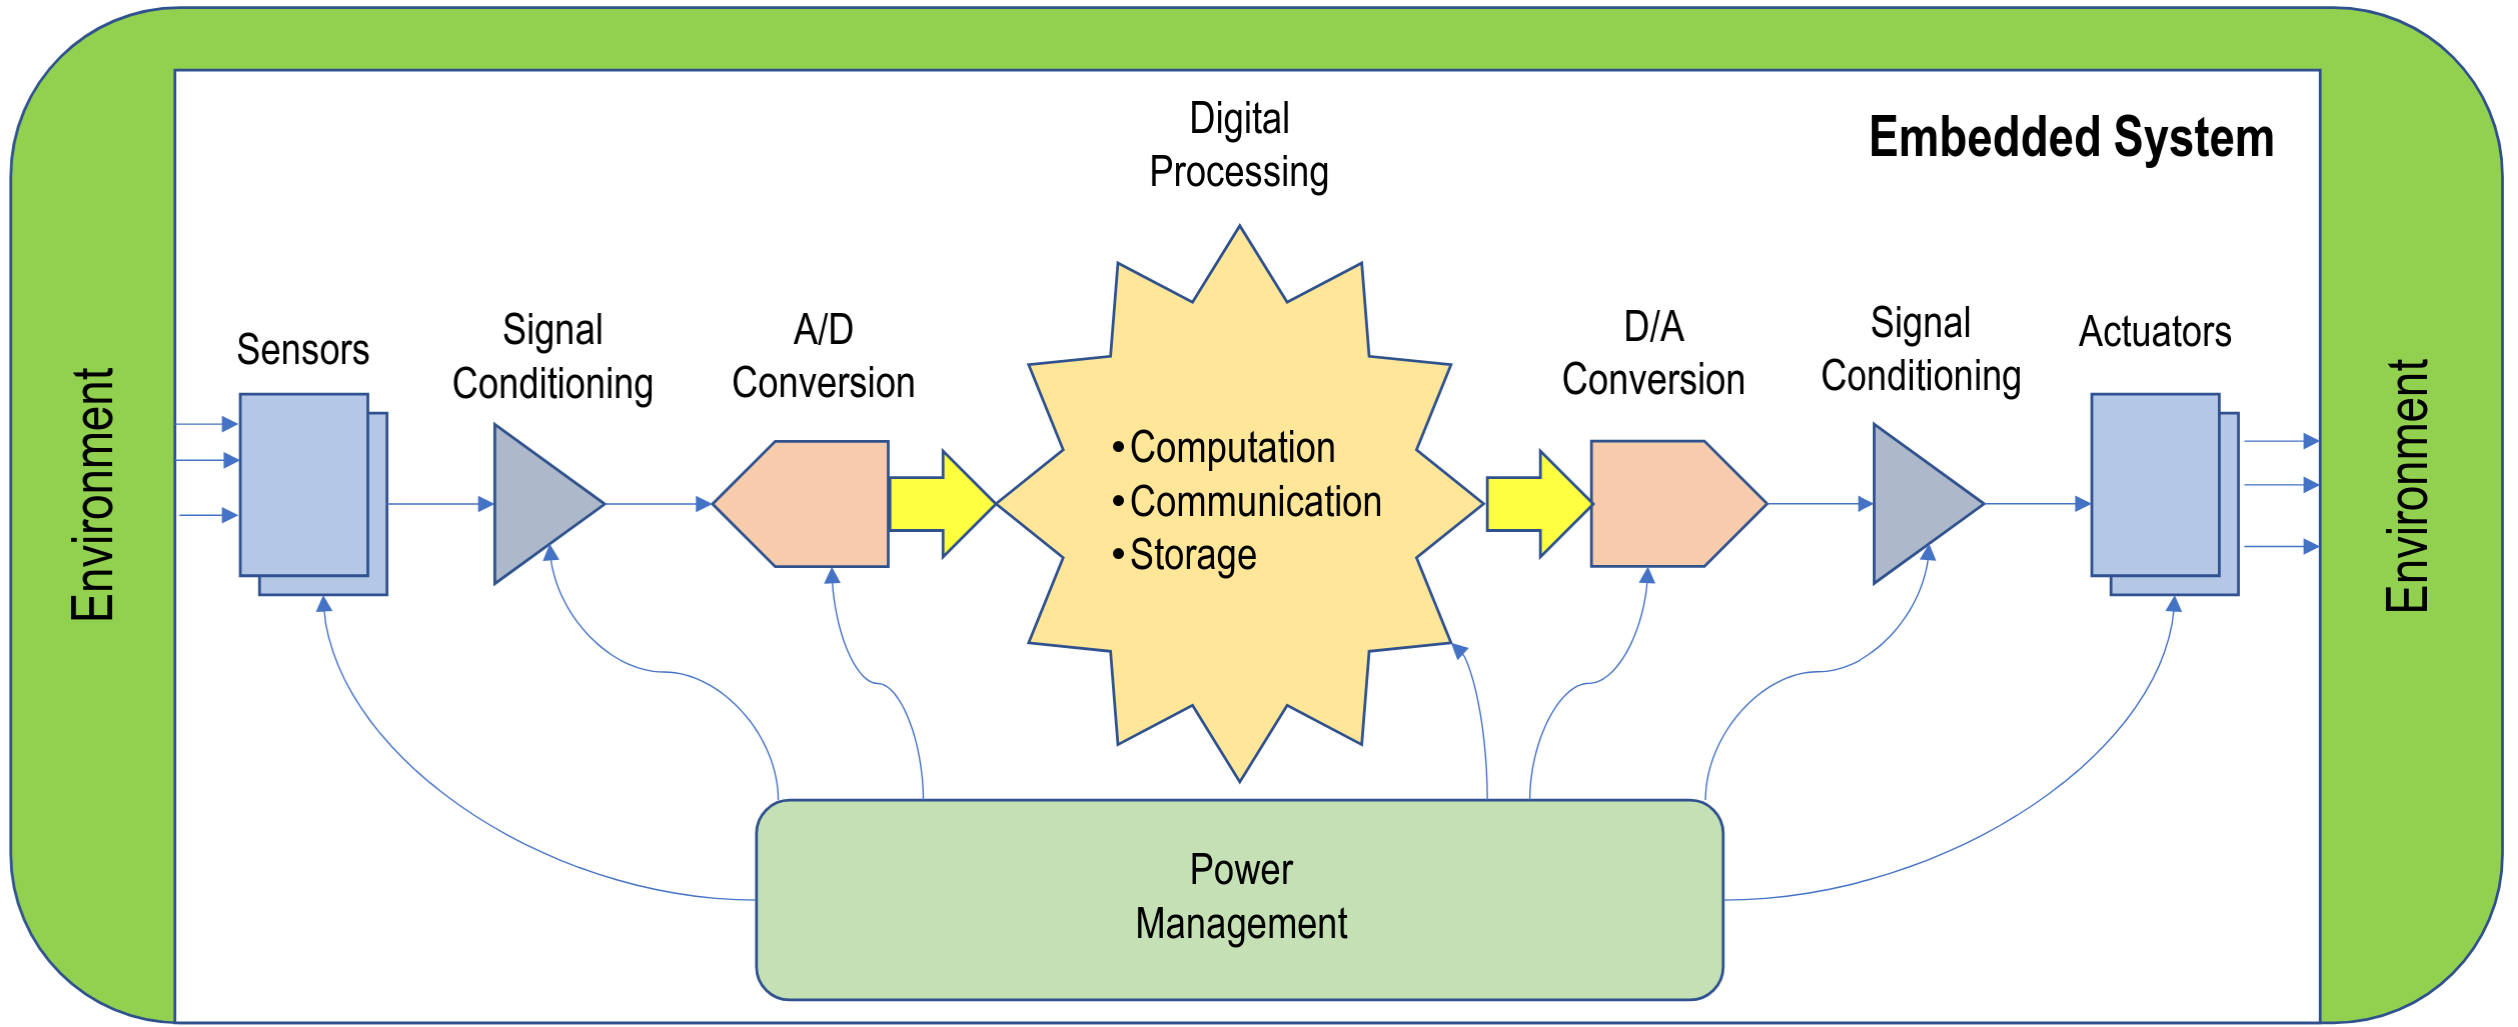
\includegraphics[scale=0.16]{../figures/emb_system.png}
\end{center}
\begin{itemize}
	\item We already know that an embedded system lives inside an \textbf{environment}, from which it \textit{senses} data and which it modifies by \textit{acting} on it;
	\item Data will be obtained from \textbf{sensors} that return electrical values proportional to physical quantities in the environment;
	\item Data will be \textbf{conditioned}, which means \textit{amplified}, \textit{filtered}, or anyways manipulated in order to be more useful to the embedded system;
	\item Data will be converted from an analog signal to a digital value ready for computation by an \textbf{A/D converter};
	\item The central part of the embedded system performs \textbf{digital processing} of the recovered data from the sensors, signal conditioning and A/D conversion parts. What comes out of this phase is digital signals which will be used to control the \textit{actuators};
	\item Data will be converted from the digital processing stage back into the analog domain by a \textbf{D/A converter};
	\item Again, we will have some amount of \textbf{conditioning} on the output signal;
	\item The conditioned signal will drive \textbf{actuators}, which can actually affect the environment;
	\item All of these components need \textbf{power management} to be correctly powered by some power supply (often batteries, but also wall power, ...).
\end{itemize}

\subsubsection{Design metrics for embedded systems}

A \textbf{design metric} is a measurable feature of a system implementation.
Common metrics are:
\begin{itemize}
	\item \textbf{Unit cost} $U$: the monetary cost of manufacturing each copy of the system;
	\item \textbf{NRE cost} $N$: one-time monetary cost of developing (designing) the system;
	\item \textbf{Total cost} $T$: total cost of producing $N_{unit}$ tests. Calculated as $T = N + U \times N_{unit}$;
	\item \textbf{Per-product cost} $p$: cost of a singular product, with amortized NRE costs. Calculated as $p = \frac{T}{N_{unit}} = \frac{N}{N_{unit}} + U$. Keeping the per-product cost low entails spending as little as possible on NRE (as these costs get amortized over units produced) or producing as many units as possible. Of course the unit cost $U$ plays a significant role: lowering is sometimes useful at the cost of increasing $N$;
	\item \textbf{Time-to-market}: it is the time required to develop a product to the point it can be sold to customers. Smaller time-to-market means less losses due to delayed market entry (for instance, when competing with other products);
	\item \textbf{Performance}: it can be measured in many ways. For instance:
		\begin{itemize}
			\item \textbf{Latency}, or \textit{response time}, the time between task start and task end;
			\item \textbf{Throughput}, taskes per second, usually $\frac{1}{\text{Latency}}$.
		\end{itemize}
		\textit{Parallelism} is a way to increase performance. Usually, $N$ parallel blocks allow to increase throughput to $N \times \text{Throughput}_\text{Serial}$ (unless Ahmdal's law comes into play);
	\item \textbf{Technologies}, that is technical processes, methods and knowledge, are in some way a design metric.
\end{itemize}

\subsubsection{Technologies}

Let's look at a few \textbf{technologies} which we have available for the design of embedded systems.
We noted the design space is very large, so it is useful to know about them. 

\par\smallskip
\textbf{\textsf{Processor technology}}

Let's look at \textbf{processor} thecnologies.

\begin{itemize}
	\item 
The \textit{General Purpose} (\textbf{GP}) processor, as found in desktop PCs, is the classic programmable micro-processor we are used to.
\begin{itemize}
	\item They are not optimized for any specific application;
	\item They are often cheaper than general purpose technology: billions of units are sold every year;
	\item Flexible, low time-to-market: software is easy to update and modify;
	\item No high performance compared to a dedicated design;
	\item Not power efficient
\end{itemize}

	\item
\textit{Embedded} micro-processors, though, are different from PC micro-processors.
For instance, they are usually within a \textit{System-On-Chip} (\textbf{SoC}), which includes needed components and a number of peripherals. 

	\item
A method of implementing embedded processors is \textit{Application Specific Instruction Processor} (\textbf{ASIP}).
This entails:
\begin{itemize}
	\item A general purpose processor with specific hardware for a certain application domain, for instance \textbf{DSP} (\textit{Digital Signal Processing});
	\item Dedicated to signal processing application;
	\item Possibly dedicated hardware to drive and read external pins;
	\item Cheap;
	\item Flexible, low time-to-market;
	\item Higher performance and better power than a GP processor.
\end{itemize}

	\item
Another method is \textit{Single Purpose} (custom) \textit{Processor}.
This entails:
\begin{itemize}
	\item Digital hardware designed specifically for a certain application;
	\item Best performance;
	\item Best power consumption;
	\item Small size;
	\item Long time-to-market;
	\item Very high NRE costs;
	\item Low flexibility;
	\item Good for large volume productions and for extremely high performance designs.
\end{itemize}
\end{itemize}

\par\smallskip
\textbf{\textsf{IC technology}}

\textbf{IC}s (\textit{Integrated Circuits}) also have different technologies with different use cases.

\begin{itemize}
	\item
		\textit{Full Custom} (\textbf{VLSI}, \textit{Very Large Scale Integration}):
\begin{itemize}
	\item The integrated circuit is entirely designed and optimized for a particular application;
	\item Transistor sizing, placing and routing;
	\item Best for performance, size and power consumption;
	\item High NRE costs;
	\item All masks in the production process are dedicated to a single design;
	\item Long time-to-market;
	\item Currently used to design micro-processors (GPs and ASIPs), memories and off-the-shelf Programmable Logic.
\end{itemize}

	\item 
		\textit{Semi-Custom} (Gate Array / Standard cells) technology:
\begin{itemize}
	\item The lower layers are fully or partially built: design entails placing of large blocks, routing;
	\item Good performance, size and power consumption;
	\item Lower NRE compared to a full custom implementation;
	\item Some masks are shared among more than one design;
	\item Still, high NRE costs (tough lower than VLSI);
	\item Long time-to-market.
\end{itemize}

\item
	\textit{Programmable Logic Device} (\textbf{PLD}):
\begin{itemize}
	\item The integrated circuit is fully built by the manufacturer: the embedded system designer buys the IC. The PLD can be customized after fabrication for a specific application;
	\item Logic functions and interconnections are programmable;
	\item Low NRE costs;
	\item Fairly good performance and power consumption, but worse than full custom and semi-custom;
	\item High unit cost;
	\item Large size.
\end{itemize}
\end{itemize}

\par\smallskip
\textbf{\textsf{Orthogonality}}

Processor and IC technologies are \textbf{orthogonal}: the design space is very large, and takes very long to explore.
We show a figure showing the different processor and IC technologies we considered, and their characteristic (low $N$ vs high $U$, or low $U$ vs high $N$).

\begin{center}
	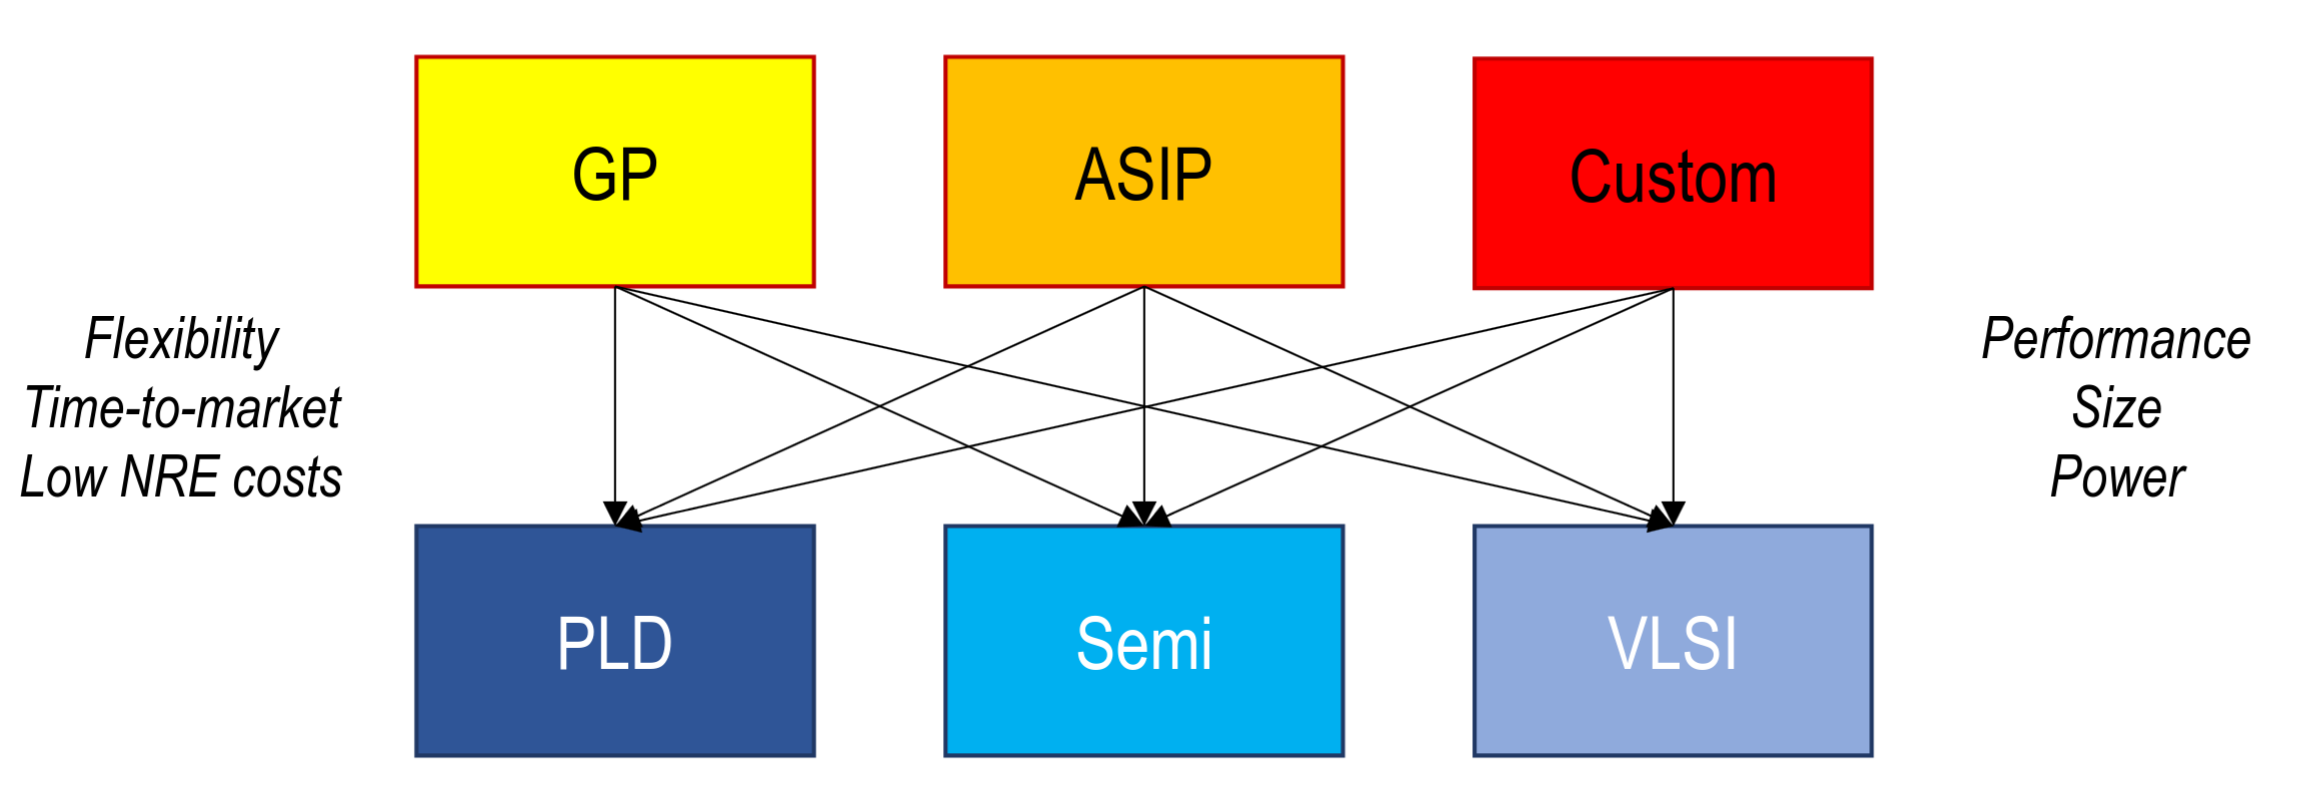
\includegraphics[scale=0.17]{../figures/ortho_tech.png}
\end{center}

Early design decisions are difficult, and it is useful to make use of modern design technologies to evaluate different solutions.

It can also be of use to note that the design phase of a product is also a field where more than one methodology (i.e. a technology and its associated techniques) can be used.
This is particularly important in companies, which might have long historical experience with one methodology instead of another.
Using well-trusted methodologies or using new ones is also an important factor to consider.

\subsection{Memories}

\textbf{Memories} are the first component of embedded systems we will encounter.
They exist in the digital domain, and more specifically in the storage component of the digital processing part of an embedded system. 

In general, there are different kinds of memory, which differ in types, operations available, interfaces, timings and composition of different memories to make bigger ones.

We know the usual types of memory:
\begin{itemize}
	\item \textbf{ROM} (\textit{Read Only Memory}), that is EPROMs, ... 
	\item \textbf{RAM} (\textit{Random Access Memory}), that is SRAM, DRAM, ...
\end{itemize}

We will also note the use of memories as \textit{cache memories} and \textit{memory controllers}.

\end{document}
